\documentclass[11pt,a4paper]{article}

% ==================== PACOTES ====================
\usepackage[utf8]{inputenc}
\usepackage[T1]{fontenc}
\usepackage[brazil]{babel}
\usepackage{geometry}
\geometry{top=2.0cm, bottom=2.2cm, left=2.0cm, right=2.0cm}
\usepackage{graphicx}
\usepackage{float}
\usepackage{hyperref}
\usepackage{enumitem}
\usepackage{booktabs}
\usepackage{array}
\usepackage{amssymb}
\usepackage{xcolor}
\usepackage{listings}
\usepackage{tcolorbox}
\tcbuselibrary{skins,breakable}

% ==================== CORES E ESTILOS ====================
\definecolor{imeblue}{RGB}{0, 51, 102}
\definecolor{alertred}{RGB}{180, 20, 20}
\definecolor{homegreen}{RGB}{20, 110, 50}
\definecolor{theorypurple}{RGB}{90, 40, 130}
\definecolor{codebg}{RGB}{245, 247, 250}

\hypersetup{
    colorlinks=true,
    linkcolor=imeblue,
    urlcolor=imeblue
}

\lstset{
    backgroundcolor=\color{codebg},
    basicstyle=\ttfamily\small,
    breaklines=true,
    frame=single,
    rulecolor=\color{gray!40},
    showstringspaces=false,
    commentstyle=\color{homegreen},
    keywordstyle=\color{imeblue}\bfseries,
    literate={á}{{\'a}}1 {à}{{\`a}}1 {ã}{{\~a}}1 {â}{{\^a}}1
             {é}{{\'e}}1 {ê}{{\^e}}1 {í}{{\'i}}1 {ó}{{\'o}}1
             {õ}{{\~o}}1 {ô}{{\^o}}1 {ú}{{\'u}}1 {ç}{{\c{c}}}1
             {Á}{{\'A}}1 {É}{{\'E}}1 {Í}{{\'I}}1 {Ó}{{\'O}}1
             {Ú}{{\'U}}1 {Ç}{{\c{C}}}1
}

% Caixas didáticas personalizadas
\newtcolorbox{alertbox}[1]{
    colback=alertred!5!white,
    colframe=alertred,
    fonttitle=\bfseries,
    title={#1},
    breakable
}

\newtcolorbox{theorybox}[1]{
    colback=theorypurple!5!white,
    colframe=theorypurple,
    fonttitle=\bfseries,
    title={#1},
    breakable
}

\newtcolorbox{homebox}[1]{
    colback=homegreen!5!white,
    colframe=homegreen,
    fonttitle=\bfseries,
    title={#1},
    breakable
}

\newtcolorbox{labbox}[1]{
    colback=imeblue!5!white,
    colframe=imeblue,
    fonttitle=\bfseries,
    title={#1},
    breakable
}

% ==================== INÍCIO DO DOCUMENTO ====================
\begin{document}

\begin{center}
    {\Large \textbf{INSTITUTO MILITAR DE ENGENHARIA (IME)}}\\[0.15cm]
    {\large Programação Aplicada à Engenharia Elétrica (SE/3 - Eletrônica)}\\[0.1cm]
    {\Large \textbf{Guia Didático Passo a Passo: Entregável 0}}\\[0.1cm]
    {\normalsize \textit{Identificação Física do Hardware, Eletrônica da Ligação e Repositório Git}}\\[0.3cm]
    \begin{tabular}{lp{10.8cm}}
        \toprule
        \textbf{Prazo Oficial (Classroom):} & \textbf{Segunda-feira, 19/10/2026 às 23:59} (Obrigatório) \\
        \textbf{Kit de Desenvolvimento:} & STMicroelectronics \textbf{STM32MP157D-DK1} (FG: \texttt{DK32MP157D1\$AU2}) \\
        \textbf{Sensor do Grupo (Nº 3):} & Módulo de Obstáculo Infravermelho Reflexivo Digital (\textbf{HW-201} / SKU: \texttt{SS10}) \\
        \textbf{Objetivo da Entrega 0:} & Foto nítida da conexão do sensor com o kit \textbf{desligado} + Estrutura Git \\
        \bottomrule
    \end{tabular}
\end{center}

\vspace{0.2cm}

% ====================================================================
\section{Cronograma Oficial Confirmado (Edital de 15/10 e Classroom)}
% ====================================================================

Com base no novo documento oficial do professor (\textit{15 de outubro de 2026}) e nas tarefas abertas no Google Classroom, este é o cronograma definitivo da disciplina:

\begin{center}
\begin{tabular}{llcp{7.8cm}}
    \toprule
    \textbf{Etapa} & \textbf{Prazo (23:59)} & \textbf{Valor} & \textbf{Descrição Oficial no Classroom / Edital} \\
    \midrule
    \textbf{Entrega 0} & \textbf{19/10/2026} (Seg) & Obrig. & Foto da conexão física do sensor com o kit \textbf{desligado}. \\
    \textbf{Entrega 1} & \textbf{26/10/2026} (Seg) & 2,0 pts & Código-fonte em C++ da classe de leitura documentada com Doxygen. \\
    \textbf{Entrega 2} & \textbf{02/11/2026} (Seg) & 2,0 pts & Programa funcional no kit + instruções de compilação/execução no \texttt{README.md}. \\
    \textbf{Entrega 3} & \textbf{09/11/2026} (Seg) & 2,0 pts & Envio da leitura via UDP para o servidor + documentação do protocolo. \\
    \textbf{Entrega 4} & \textbf{16/11/2026} (Seg) & 2,0 pts & Interface gráfica no PC (tempo real, histórico 30--60s e log/CSV). \\
    \textbf{Entrega 5} & \textbf{16/11/2026} (Seg) & 2,0 pts & \textbf{Atenção: Mesmo dia da Entrega 4!} Vídeo de demonstração, apresentação e documentação completa no \texttt{README.md}. \\
    \bottomrule
\end{tabular}
\end{center}

\begin{figure}[H]
    \centering
    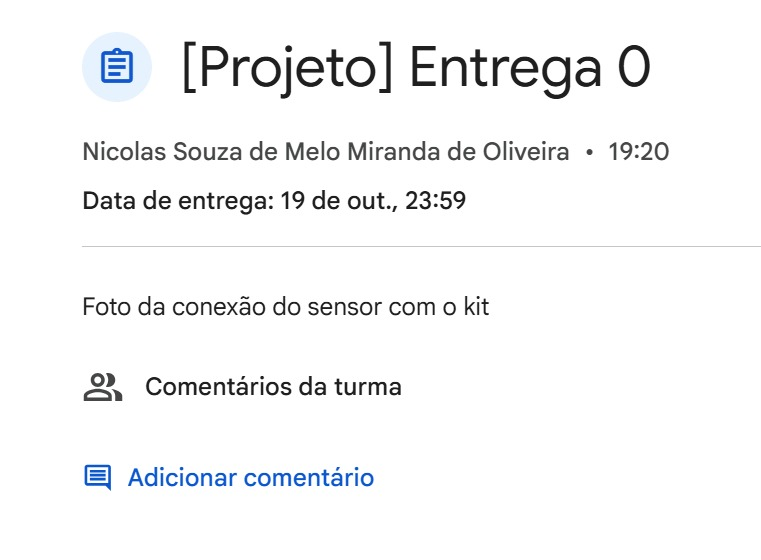
\includegraphics[width=0.62\textwidth]{latex_assets/classroom_entrega0.jpg}
    \caption{Tarefa oficial aberta no Google Classroom da SE/3 para a Entrega 0.}
\end{figure}

% ====================================================================
\section{Conhecendo o Hardware que Você Recebeu}
% ====================================================================

Antes de conectar qualquer fio, um engenheiro precisa conhecer exatamente as especificações elétricas dos componentes que tem em mãos. Pelas fotos das embalagens recebidas pelo seu grupo, temos dois elementos principais:

\begin{figure}[H]
    \centering
    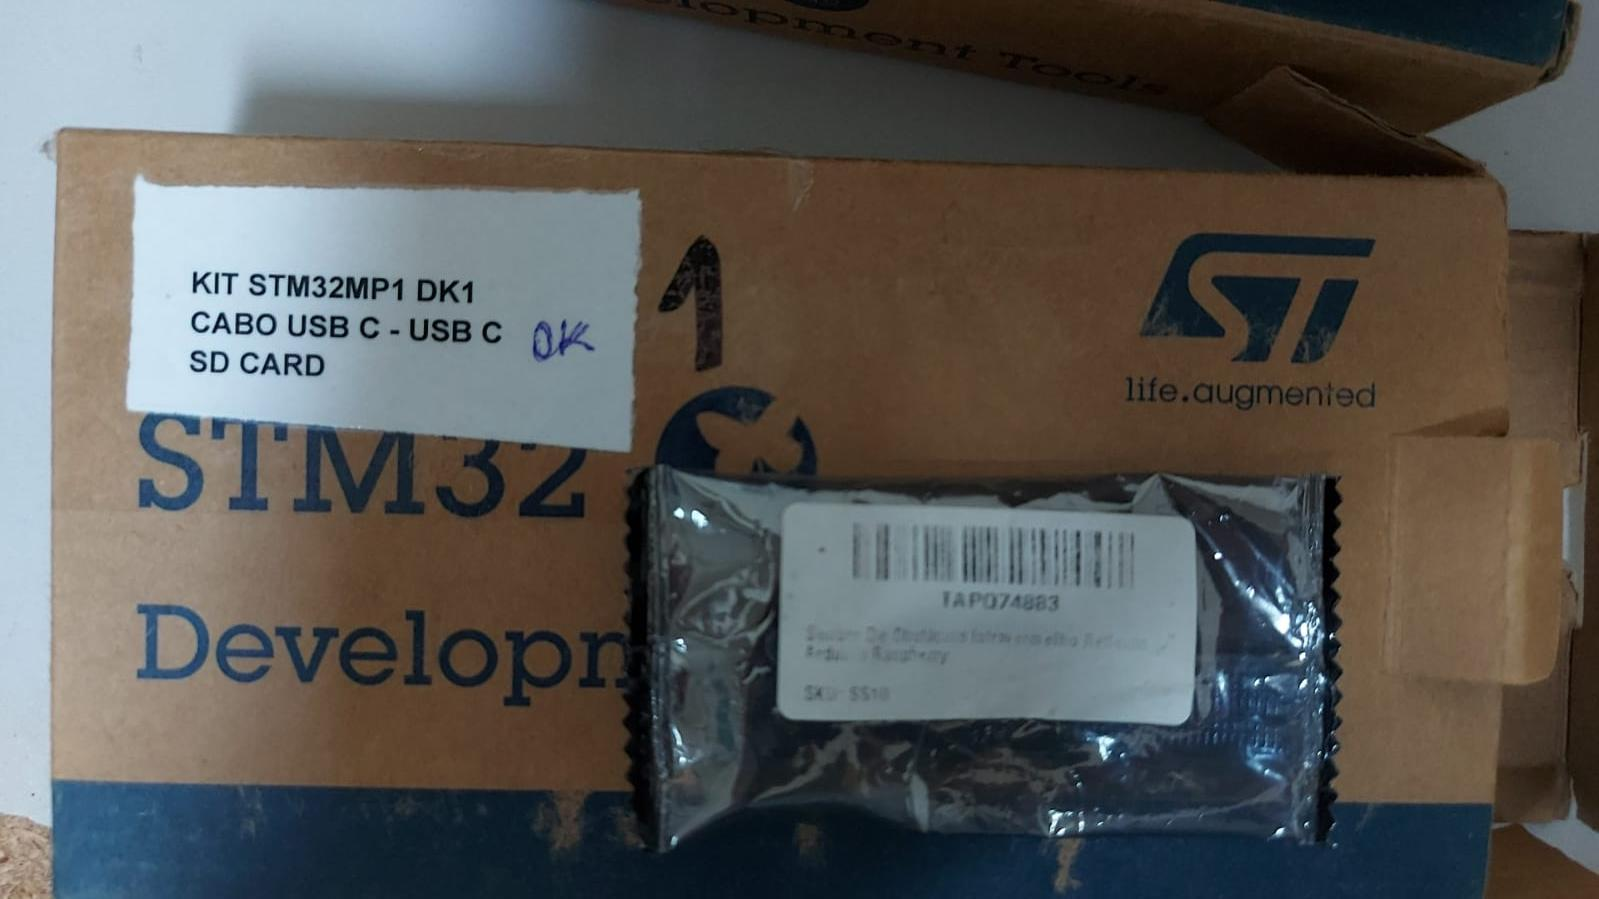
\includegraphics[height=4.8cm]{latex_assets/foto_kit_caixa.jpg}
    \hspace{0.4cm}
    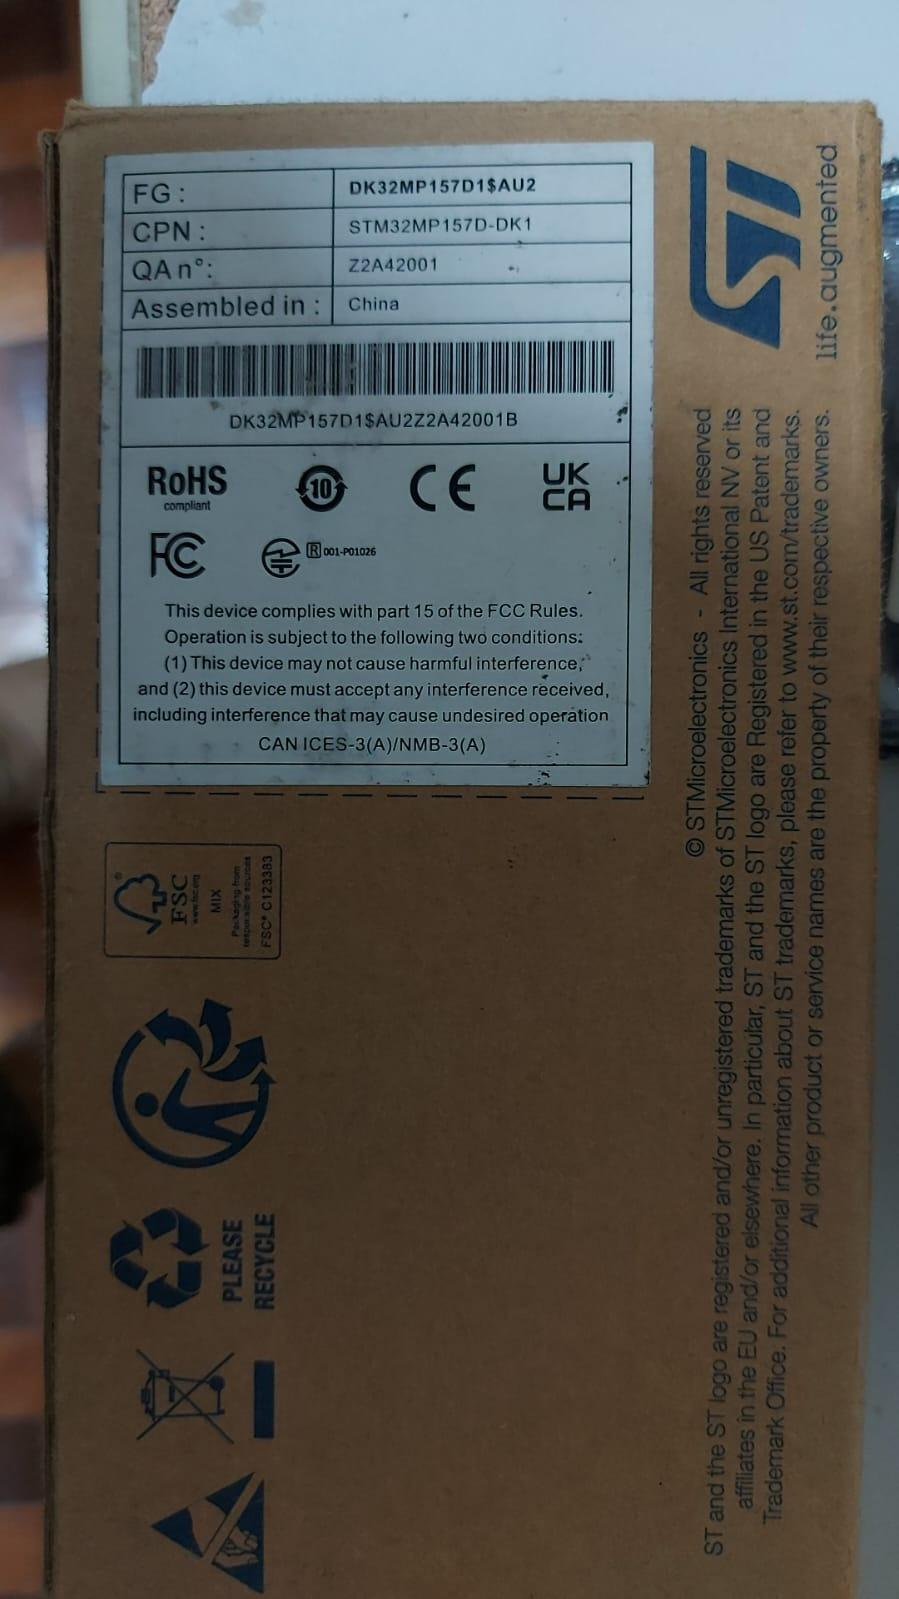
\includegraphics[height=4.8cm]{latex_assets/foto_etiqueta_stm32.jpg}
    \caption{Fotos reais do kit recebido pelo grupo: Caixa com etiqueta de conferência (\texttt{KIT STM32MP1 DK1 + CABO USB C + SD CARD}), saquinho do sensor infravermelho (\texttt{SKU: SS10}) e etiqueta lateral da STMicroelectronics (\texttt{CPN: STM32MP157D-DK1}).}
\end{figure}

\subsection{A Placa: STMicroelectronics STM32MP157D-DK1}
Diferente de um Arduino ou de um STM32 tradicional (que possuem apenas um microcontrolador simples), a sua placa é um sistema computacional completo baseado no chip híbrido \textbf{STM32MP157DAC1}:
\begin{itemize}[leftmargin=*]
    \item \textbf{Dual Arm Cortex-A7 (800 MHz):} É um microprocessador de aplicação (como o de um smartphone ou Raspberry Pi) que roda uma distribuição completa do \textbf{Sistema Operacional Linux} (gravada no cartão microSD da placa). \textbf{É aqui que o seu programa em C++ vai rodar!}
    \item \textbf{Arm Cortex-M4 (209 MHz):} Um microcontrolador interno dedicado a tempo real.
    \item \textbf{Nível Lógico de 3,3 V:} Todos os pinos de entrada e saída (GPIOs e conversores Analógico-Digitais) operam com tensão máxima de \textbf{3,3 V}.
\end{itemize}

\subsection{O Sensor: Módulo Infravermelho Reflexivo (HW-201 / LM393)}
O seu grupo recebeu o \textbf{Sensor Nº 3 do edital}, cuja missão no projeto de \textit{Monitoramento Inteligente de Carga} é detectar a aproximação ou a abertura não autorizada do compartimento da carga.

\begin{theorybox}{Por dentro do Sensor: Como a Física vira Sinal Elétrico?}
Na ponta do seu sensor HW-201 existem dois componentes parecidos com LEDs de 5 mm:
\begin{enumerate}[leftmargin=*]
    \item \textbf{Emissor Infravermelho (transparente):} Quando o sensor é alimentado, ele emite um feixe contínuo de luz infravermelha (invisível ao olho humano).
    \item \textbf{Fototransistor Receptor (preto):} Fica ao lado do emissor e só conduz corrente elétrica quando a luz infravermelha bate em um obstáculo (como a tampa da caixa de carga) e \textbf{reflete de volta} para ele.
    \item \textbf{Circuito Integrado LM393 e Trimpot Azul:} O chip LM393 é um \textit{comparador de tensão}. Ele compara a quantidade de luz refletida no receptor com a referência ajustada no parafuso do potenciômetro quadrado azul (trimpot, que ajusta o alcance entre 2 cm e 30 cm):
    \begin{itemize}
        \item \textbf{Sem obstáculo (feixe se perde no ar):} O pino de saída \texttt{OUT} fica em \textbf{Nível Lógico ALTO (3,3 V)}.
        \item \textbf{Com obstáculo (feixe reflete de volta):} O pino de saída \texttt{OUT} cai para \textbf{Nível Lógico BAIXO (0 V)} e o LED indicador na placa do sensor acende (\textit{lógica Active-Low}).
    \end{itemize}
\end{enumerate}
\end{theorybox}

% ====================================================================
\section{Os ``Porquês'' Elétricos da Conexão (Segurança de Bancada)}
% ====================================================================

\begin{alertbox}{Três Perguntas que Todo Aluno Faz (e que Salvam a Placa)}
\begin{enumerate}[leftmargin=*]
    \item \textbf{Por que é PROIBIDO ligar o sensor no pino de 5V da placa?} \\
    O sensor HW-201 aceita de 3,3 V a 5 V. Porém, a tensão que ele solta no pino de saída (\texttt{OUT}) quando está em nível ALTO é igual à tensão com que ele foi alimentado no \texttt{VCC}. Se você alimentar o sensor com \textbf{5 V}, ele jogará \textbf{5 V} dentro do pino de leitura do processador STM32MP157D, que suporta no máximo \textbf{3,3 V}. Isso queima o conversor A/D da placa instantaneamente! Ao alimentar o sensor com \textbf{3,3 V}, a saída \texttt{OUT} varia apenas entre \textbf{0 V e 3,3 V}, protegendo 100\% o kit.
    
    \item \textbf{Se o sensor HW-201 tem saída digital (0 ou 1), por que vamos ligá-lo no pino Analógico (ADC)?} \\
    Porque o roteiro oficial do professor padronizou que todos os sensores de pinos simples (analógicos ou digitais) sejam lidos através do conversor Analógico-Digital (ADC) gerenciado pelo subsistema \textbf{IIO (Industrial I/O)} do Linux (\texttt{/sys/bus/iio/devices/iio:device0/in\_voltageX\_raw}). Na prática, quando a saída for 0 V, o ADC lerá um número próximo de \texttt{0}; quando for 3,3 V, lerá o valor máximo da escala do conversor!
    
    \item \textbf{Por que não posso tirar o cartão microSD nem ligar o cabo USB antes da foto?} \\
    O cartão microSD contém todo o sistema operacional Linux pré-configurado pelo professor. E a foto da Entrega 0 com a placa \textbf{desligada} serve justamente para o professor conferir visualmente se você não espetou nenhum fio no pino de 5V ou em curto-circuito antes de energizar!
\end{enumerate}
\end{alertbox}

\newpage
% ====================================================================
\section{Parte 1: O que Fazer em CASA (Git, GitHub e README)}
% ====================================================================

Como o kit fica no laboratório, você já pode deixar toda a parte de software e documentação da Entrega 0 pronta de casa.

\begin{homebox}{Passo a Passo em Casa --- Configurando o Repositório do Grupo}
\textbf{1. Criar o Repositório Online no GitHub:}
\begin{itemize}[leftmargin=*]
    \item Acesse \url{https://github.com} e crie um novo repositório (ex.: \texttt{projeto-prog-aplicada-stm32}).
    \item \textbf{Importante:} Marque a visibilidade como \textbf{Public (Público)} para que o professor consiga abrir o link do commit enviado no Google Classroom sem barreiras de permissão.
    \item Vá em \textbf{Settings $\rightarrow$ Collaborators $\rightarrow$ Add people} e adicione os outros dois integrantes do seu grupo.
\end{itemize}

\textbf{2. Clonar no seu PC e Criar a Estrutura de Pastas:} \\
Abra o terminal na sua pasta de estudos e execute os comandos abaixo (compreendendo o que cada um faz):
\begin{lstlisting}[language=bash]
# Clona o repositorio recem-criado para o seu computador
git clone https://github.com/SEU_USUARIO/NOME_DO_REPO.git
cd NOME_DO_REPO

# Cria as pastas organizadas para o projeto:
# include/ -> para os cabecalhos (.hpp) da Entrega 1
# src/     -> para os codigos-fonte (.cpp) da Entrega 1
# docs/    -> para guardar a foto da Entrega 0 e futuros prints
mkdir include src docs
\end{lstlisting}

\textbf{3. Escrever a estrutura inicial do \texttt{README.md}:} \\
Segundo a Instrução Geral nº 5 do edital, o arquivo \texttt{README.md} na raiz do repositório deve ser atualizado a cada entrega. Abra o \texttt{README.md} no seu editor de texto e escreva com as suas palavras:
\begin{itemize}[leftmargin=*]
    \item \textbf{Título do Projeto e Integrantes do Grupo.}
    \item \textbf{Descrição Geral:} Explique o cenário de monitoramento de carga militar usando a placa \texttt{STM32MP157D-DK1} e o sensor infravermelho reflexivo \texttt{HW-201} (explicando como ele detecta a abertura/violação do compartimento).
    \item \textbf{Seção ``Entrega 0 --- Conexão Física'':} Crie uma tabela indicando onde cada um dos 3 pinos do sensor foi conectado na placa e deixe a linha \texttt{![Conexão Física](docs/entrega0\_conexao.jpg)} pronta esperando a foto que você tirará no laboratório.
\end{itemize}
\end{homebox}

% ====================================================================
\section{Parte 2: O que Fazer no LABORATÓRIO (Montagem Física)}
% ====================================================================

Chegando ao laboratório, você precisará de apenas \textbf{10 a 15 minutos} com o kit em mãos para executar a montagem física e fotografar.

\subsection{Materiais Necessários na Bancada}
\begin{itemize}[leftmargin=*]
    \item Placa \textbf{STM32MP157D-DK1} (fora da caixa, sobre uma superfície isolante/não metálica).
    \item Módulo Sensor Infravermelho \textbf{HW-201} (fora do saquinho antiestático).
    \item \textbf{3 cabos jumper Fêmea-Macho} (preferencialmente nas cores \textbf{Vermelho}, \textbf{Marrom/Preto} e \textbf{Laranja/Amarelo}, iguais aos da figura do professor para facilitar a correção visual).
    \item Celular com câmera para tirar a foto nítida.
\end{itemize}

\begin{figure}[H]
    \centering
    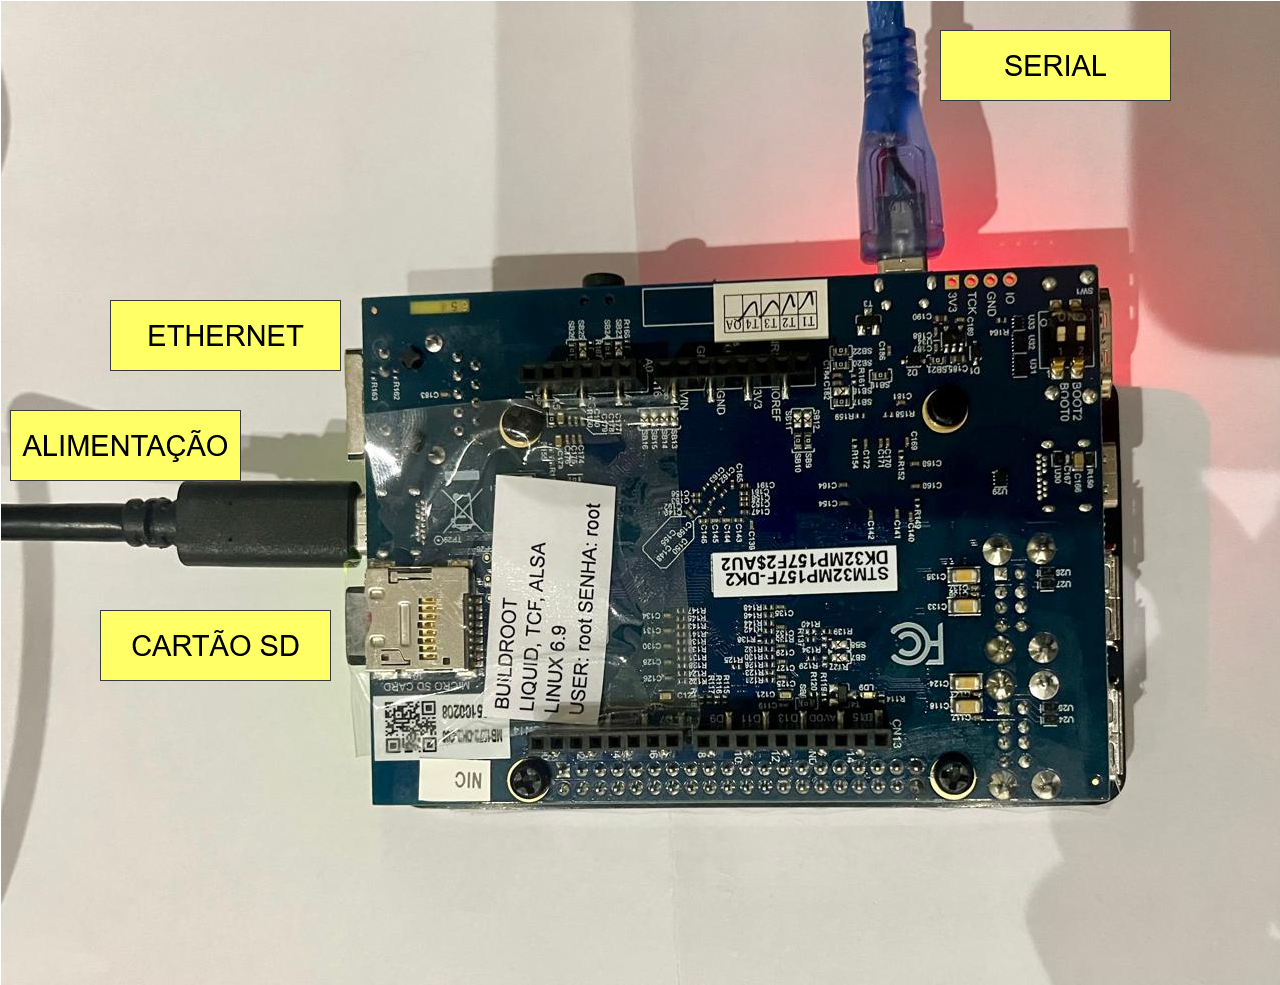
\includegraphics[width=0.72\textwidth]{latex_assets/page6_img1.png}
    \caption{Vista geral da parte traseira da placa STM32MP1-DK1 (Figura 2 do roteiro). Repare na posição do Cartão SD à esquerda e nas duas fileiras pretas de conectores na parte inferior.}
\end{figure}

\subsection{Roteiro de Ligação Pino a Pino (Siga na Ordem)}

\begin{labbox}{Execução Prática no Laboratório --- Entrega 0}
\textbf{PASSO 1: Verificação de Desligamento Total} \\
Confira se \textbf{NENHUM cabo USB} (nem o USB-C de energia, nem o Micro-USB serial, nem o cabo de rede Ethernet) está plugado na placa. A placa deve estar 100\% desligada.

\vspace{0.2cm}
\textbf{PASSO 2: Conectar as Pontas Fêmeas nos 3 Pinos do Sensor HW-201} \\
Olhe para a plaquinha do sensor HW-201 e leia a serigrafia (letras impressas ao lado dos 3 pinos metálicos):
\begin{itemize}[leftmargin=*]
    \item Espete a ponta fêmea do jumper \textbf{Vermelho} no pino escrito \textbf{\texttt{VCC}}.
    \item Espete a ponta fêmea do jumper \textbf{Marrom (ou Preto)} no pino escrito \textbf{\texttt{GND}}.
    \item Espete a ponta fêmea do jumper \textbf{Laranja} no pino escrito \textbf{\texttt{OUT}} (ou \texttt{D0}).
\end{itemize}

\vspace{0.2cm}
\textbf{PASSO 3: Posicionar a Placa STM32MP157D-DK1 na Bancada} \\
Vire a placa de costas (lado azul com o adesivo branco \texttt{USER: root SENHA: root} virado para cima), deixando os \textbf{conectores pretos fêmea na borda inferior (mais próxima de você)} e o \textbf{slot do cartão microSD apontando para a esquerda}, exatamente como nas fotos da página seguinte.

\vspace{0.2cm}
\textbf{PASSO 4: Conectar a Alimentação (\texttt{3V3} e \texttt{GND}) no Conector da Direita (8 furos)} \\
Localize o bloco preto de \textbf{8 furos à direita} (onde estão escritas na placa as siglas \texttt{IOREF}, \texttt{3V3}, \texttt{GND}, \texttt{VIN}). \textbf{Conte os furos da DIREITA para a ESQUERDA (de 1 até 8):}
\begin{itemize}[leftmargin=*]
    \item Furos 1, 2 e 3: \textit{Deixe vazios}.
    \item \textbf{Furo 4 (acima da inscrição \texttt{3V3}):} Espete a ponta macho do fio \textbf{Vermelho (\texttt{VCC})}.
    \item Furos 5 e 6: \textit{Deixe vazios}.
    \item \textbf{Furo 7 (acima da inscrição \texttt{GND}, ao lado de \texttt{VIN}):} Espete a ponta macho do fio \textbf{Marrom/Preto (\texttt{GND})}.
    \item Furo 8 (\texttt{VIN}): \textit{Deixe vazio}.
\end{itemize}

\vspace{0.2cm}
\textbf{PASSO 5: Conectar o Sinal (\texttt{OUT}) no Conector da Esquerda (6 furos --- ADC)} \\
Agora olhe para o bloco preto de \textbf{6 furos logo à esquerda} do anterior (são as portas analógicas \texttt{A0} a \texttt{A5}). \textbf{Conte também da DIREITA para a ESQUERDA (de 1 até 6):}
\begin{itemize}[leftmargin=*]
    \item Furos 1, 2, 3 e 4: \textit{Deixe vazios}.
    \item \textbf{Furo 5 (penúltimo furo da direita para a esquerda):} Espete a ponta macho do fio \textbf{Laranja (\texttt{SINAL / OUT})}.
    \item Furo 6 (último na ponta esquerda): \textit{Deixe vazio}.
\end{itemize}
\end{labbox}

\begin{figure}[H]
    \centering
    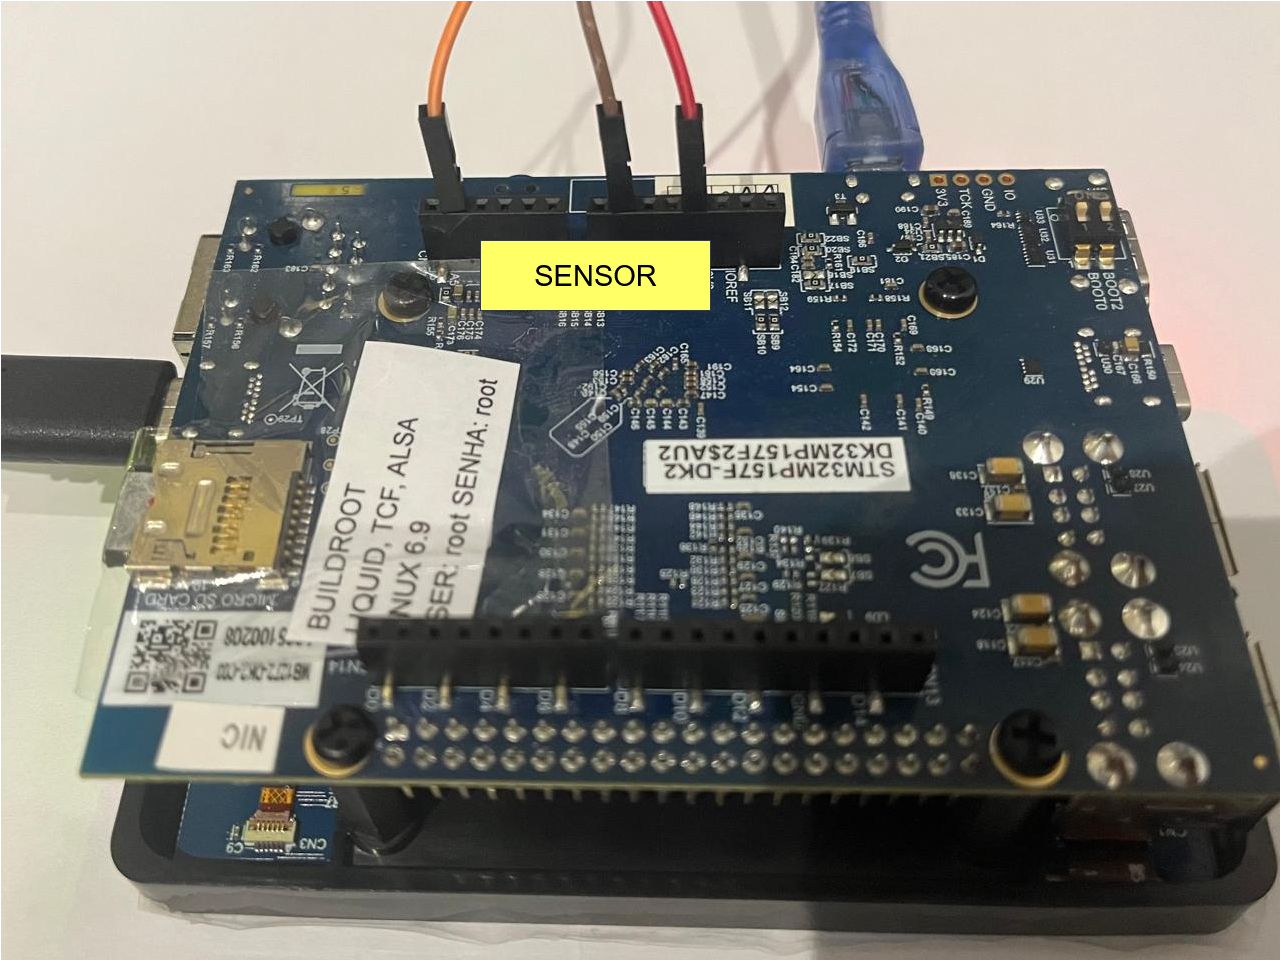
\includegraphics[width=0.47\textwidth]{latex_assets/page9_img1.png}
    \hfill
    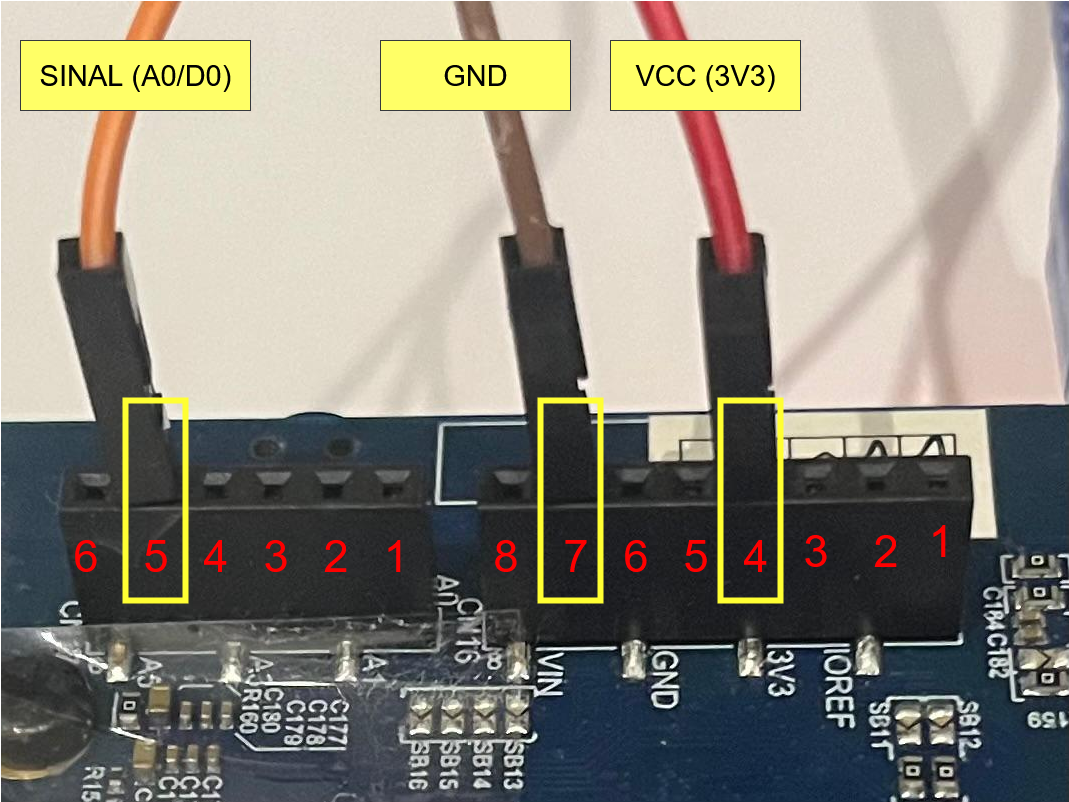
\includegraphics[width=0.49\textwidth]{latex_assets/page9_img2.png}
    \caption{Referência visual obrigatória (Figuras 4 e 5 do PDF do professor): À esquerda, a visão geral com a placa desligada e o sensor conectado. À direita, o zoom com a contagem exata dos furos \textbf{da direita para a esquerda}: \textbf{Pino 4 = VCC (3V3)}, \textbf{Pino 7 = GND} no bloco de 8 furos, e \textbf{Pino 5 = SINAL (A0/D0)} no bloco de 6 furos.}
\end{figure}

% ====================================================================
\section{Conferência Final, Foto e Submissão da Entrega 0}
% ====================================================================

Antes de tirar a foto e finalizar a Entrega 0, passe o olho neste checklist de verificação:

\begin{center}
\begin{tabular}{ccccp{5.4cm}}
    \toprule
    \textbf{Check} & \textbf{Sinal} & \textbf{Cor} & \textbf{Bloco / Pino} & \textbf{Como Conferir Visualmente na Placa} \\
    \midrule
    $\square$ & \texttt{VCC} & Vermelho & Direita (8 furos) --- \textbf{Pino 4} & Há 3 furos vazios à direita dele; na placa está escrito \texttt{3V3}. \\
    $\square$ & \texttt{GND} & Marrom/Preto & Direita (8 furos) --- \textbf{Pino 7} & Há 2 furos vazios entre ele e o fio vermelho, e sobra 1 furo vazio à esquerda dele (\texttt{VIN}). \\
    $\square$ & \texttt{OUT} & Laranja & Esquerda (6 furos) --- \textbf{Pino 5} & Há 4 furos vazios à direita dele e sobra apenas 1 furo vazio na ponta esquerda. \\
    \bottomrule
\end{tabular}
\end{center}

\subsection{Como Fotografar e Enviar (Até 19/10 às 23:59)}
\begin{enumerate}[leftmargin=*]
    \item \textbf{Tire duas fotos bem iluminadas e focadas:} Uma mostrando o conjunto inteiro (a placa desligada sem cabos USB + os 3 fios + o sensor HW-201, igual à Figura 4) e outra mais aproximada nos conectores pretos (igual à Figura 5) para não deixar nenhuma dúvida na correção.
    \item \textbf{Suba para o GitHub do Grupo:}
    \begin{lstlisting}[language=bash]
# Copie a foto para a pasta docs/ do seu repositorio
cp caminho/da/foto.jpg docs/entrega0_conexao.jpg

# Adicione os arquivos, crie o commit da Entrega 0 e envie para o GitHub
git add docs/entrega0_conexao.jpg README.md
git commit -m "Entrega 0: Conexao fisica do sensor HW-201 na STM32MP157D-DK1"
git push origin main
    \end{lstlisting}
    \item \textbf{Envie no Google Classroom:} Na tarefa \texttt{[Projeto] Entrega 0}, anexe a foto nítida da conexão (e cole também o link do repositório/commit se desejar). \textbf{Aguarde a validação do professor antes de ligar a placa na tomada!}
\end{enumerate}

\end{document}
